

\subsection{Core Algorithm}
\label{subsec::algorithm}

Algorithm~\ref{alg:bucket-cvrp} presents our Bucket-Partitioned MDS (BP-MDS), a divide-and-conquer parallel and memory-efficient algorithm. The method is governed by two key parameters: the angular partitioning parameter $\alpha$, which controls the number of spatial decompositions, and the exploration parameter $\rho$, which governs the diversity of route constructions. The algorithm takes these two parameters, $\alpha$ and $\rho$, as inputs and produces a feasible, high-quality approximate solution to the CVRP.

\textbf{Divide CVRP:} BP-MDS partitions the two-dimensional plane into angular regions (Line~\ref{alg:bucket-cvrp:line2}) centered at the depot. Customers are assigned to their respective regions based on their angular positions, and together with the depot, are grouped into buckets (Fig.~\ref{fig:2-d-partition}). This step is implemented via the \textsc{Get\_Buckets} procedure (Algorithm~\ref{alg:get-buckets}, detailed in Section~\ref{subsec:create_buckets}). Within each bucket, we conceptually model a complete graph over the assigned vertices without explicitly materializing all the edges.

\textbf{Conquer CVRP in Parallel:} BP-MDS processes each bucket independently in parallel (Lines~\ref{alg:bucket-cvrp:line3}--\ref{alg:bucket-cvrp:line22}), forming the core conquer phase of the algorithm. For every bucket, we construct a Minimum Spanning Tree (MST) over its vertices (Line~\ref{alg:bucket-cvrp:line4}) using \textsc{Construct\_MST} (Algorithm~\ref{alg:construct-mst}, detailed in Section~\ref{subsec:construct_mst}), which provides a sparse backbone for route generation. To explore diverse routing configurations, we perform $\rho$ independent iterations in parallel (Lines~\ref{alg:bucket-cvrp:line6}--\ref{alg:bucket-cvrp:line13}), each generating a candidate solution via a randomized depth-first traversal of the MST (Algorithm~\ref{alg:get-routes-from-random-dfs}, detailed in Section~\ref{subsec:routes_construction_via_random_DFS}). Within each partition, additional parallelism is exploited by spawning sub-threads to solve the corresponding subproblems using different route orderings induced by $\rho$. This results in a hierarchical (multi-level or nested) parallelization scheme. Among the generated candidates, the minimum-cost solution is selected for subsequent processing using a critical section (Line~\ref{alg:bucket-cvrp:line8}) to safely update the shared variables ($min\_cost\_routes$ and $min\_cost$).
Finally, the partial solutions obtained from all the partitions are refined (Line~\ref{alg:bucket-cvrp:line17}) through intra-route optimization using 2-opt~\cite{Croes_1958, Flood_1956} and the nearest-neighbor heuristics~\cite{Rosenkrantz_1977}, following the approach of Muniasamy et al.~\cite{Muniasamy_VRP} to improve the solution quality. These refined routes are then combined in a consolidation phase to construct a complete feasible solution in a critical section (Lines~\ref{alg:bucket-cvrp:line18}--\ref{alg:bucket-cvrp:line21}) %to avoid race conditions, 
as both the global route container and the total cost are shared across concurrently running worker threads. 



\begin{algorithm}
\caption{\textsc{Bucket\_Partitioned\_MDS}}
\label{alg:bucket-cvrp}
\SetEndCharOfAlgoLine{}
\SetAlgoLined

\KwIn{CVRP instance, parameters $\alpha$, $\rho$}
\KwOut{$routes$: feasible CVRP solution; $cost$: total cost}

$final\_routes \gets \emptyset$, $final\_cost \gets 0$\;  \label{alg:bucket-cvrp:line1}

\tcp{Divide CVRP}
$buckets \leftarrow \textsc{Get\_Buckets}(CVRP, \alpha)$  \label{alg:bucket-cvrp:line2}


\For{bucket in buckets \textbf{in parallel}} { \label{alg:bucket-cvrp:line3}

    $T \leftarrow \textsc{Construct\_MST}(CVRP, bucket)$\;                                              \label{alg:bucket-cvrp:line4}
    
    $min\_cost\_routes \leftarrow \emptyset$, $min\_cost \leftarrow \infty$\;                           \label{alg:bucket-cvrp:line5}
    
    \tcp{Exploit the MST by exploring multiple DFS orderings}
    \For{$\rho$ iterations \textbf{in parallel}}{  \label{alg:bucket-cvrp:line6}
        $(routes, cost) \leftarrow \textsc{Get\_Routes\_From\_Random\_DFS}(CVRP, T, bucket)$\; \label{alg:bucket-cvrp:line7}

        \Critical{                                                                                      \label{alg:bucket-cvrp:line8}
            \If{$cost < min\_cost$}{                                                                    \label{alg:bucket-cvrp:line9}
                $min\_cost\_routes \leftarrow routes$, $min\_cost \leftarrow cost$\;                                                           \label{alg:bucket-cvrp:line10}
            } \label{alg:bucket-cvrp:line11}
        } \label{alg:bucket-cvrp:line12}
    } \label{alg:bucket-cvrp:line13}

    \tcp{Refine and combine routes from all partitions}
    $(refined\_routes, refined\_cost) \leftarrow \textsc{Refine\_Routes}(CVRP, min\_cost\_routes)$\;    \label{alg:bucket-cvrp:line17}
    \Critical{                                                                                          \label{alg:bucket-cvrp:line18}
        $final\_routes \leftarrow final\_routes \cup refined\_routes$\;                                 \label{alg:bucket-cvrp:line19}
        $final\_cost \leftarrow final\_cost + refined\_cost$\;                                          \label{alg:bucket-cvrp:line20}
    }                                                                                                   \label{alg:bucket-cvrp:line21}
}                                                                                                       \label{alg:bucket-cvrp:line22}
\Return{$(final\_routes, final\_cost)$}                                                                 \label{alg:bucket-cvrp:line23}

\end{algorithm}






% \begin{figure*}[htbp]
%     \centering
%     \caption{Multi-level Multi-threading}
%     \label{fig:multi-level-threading}
%     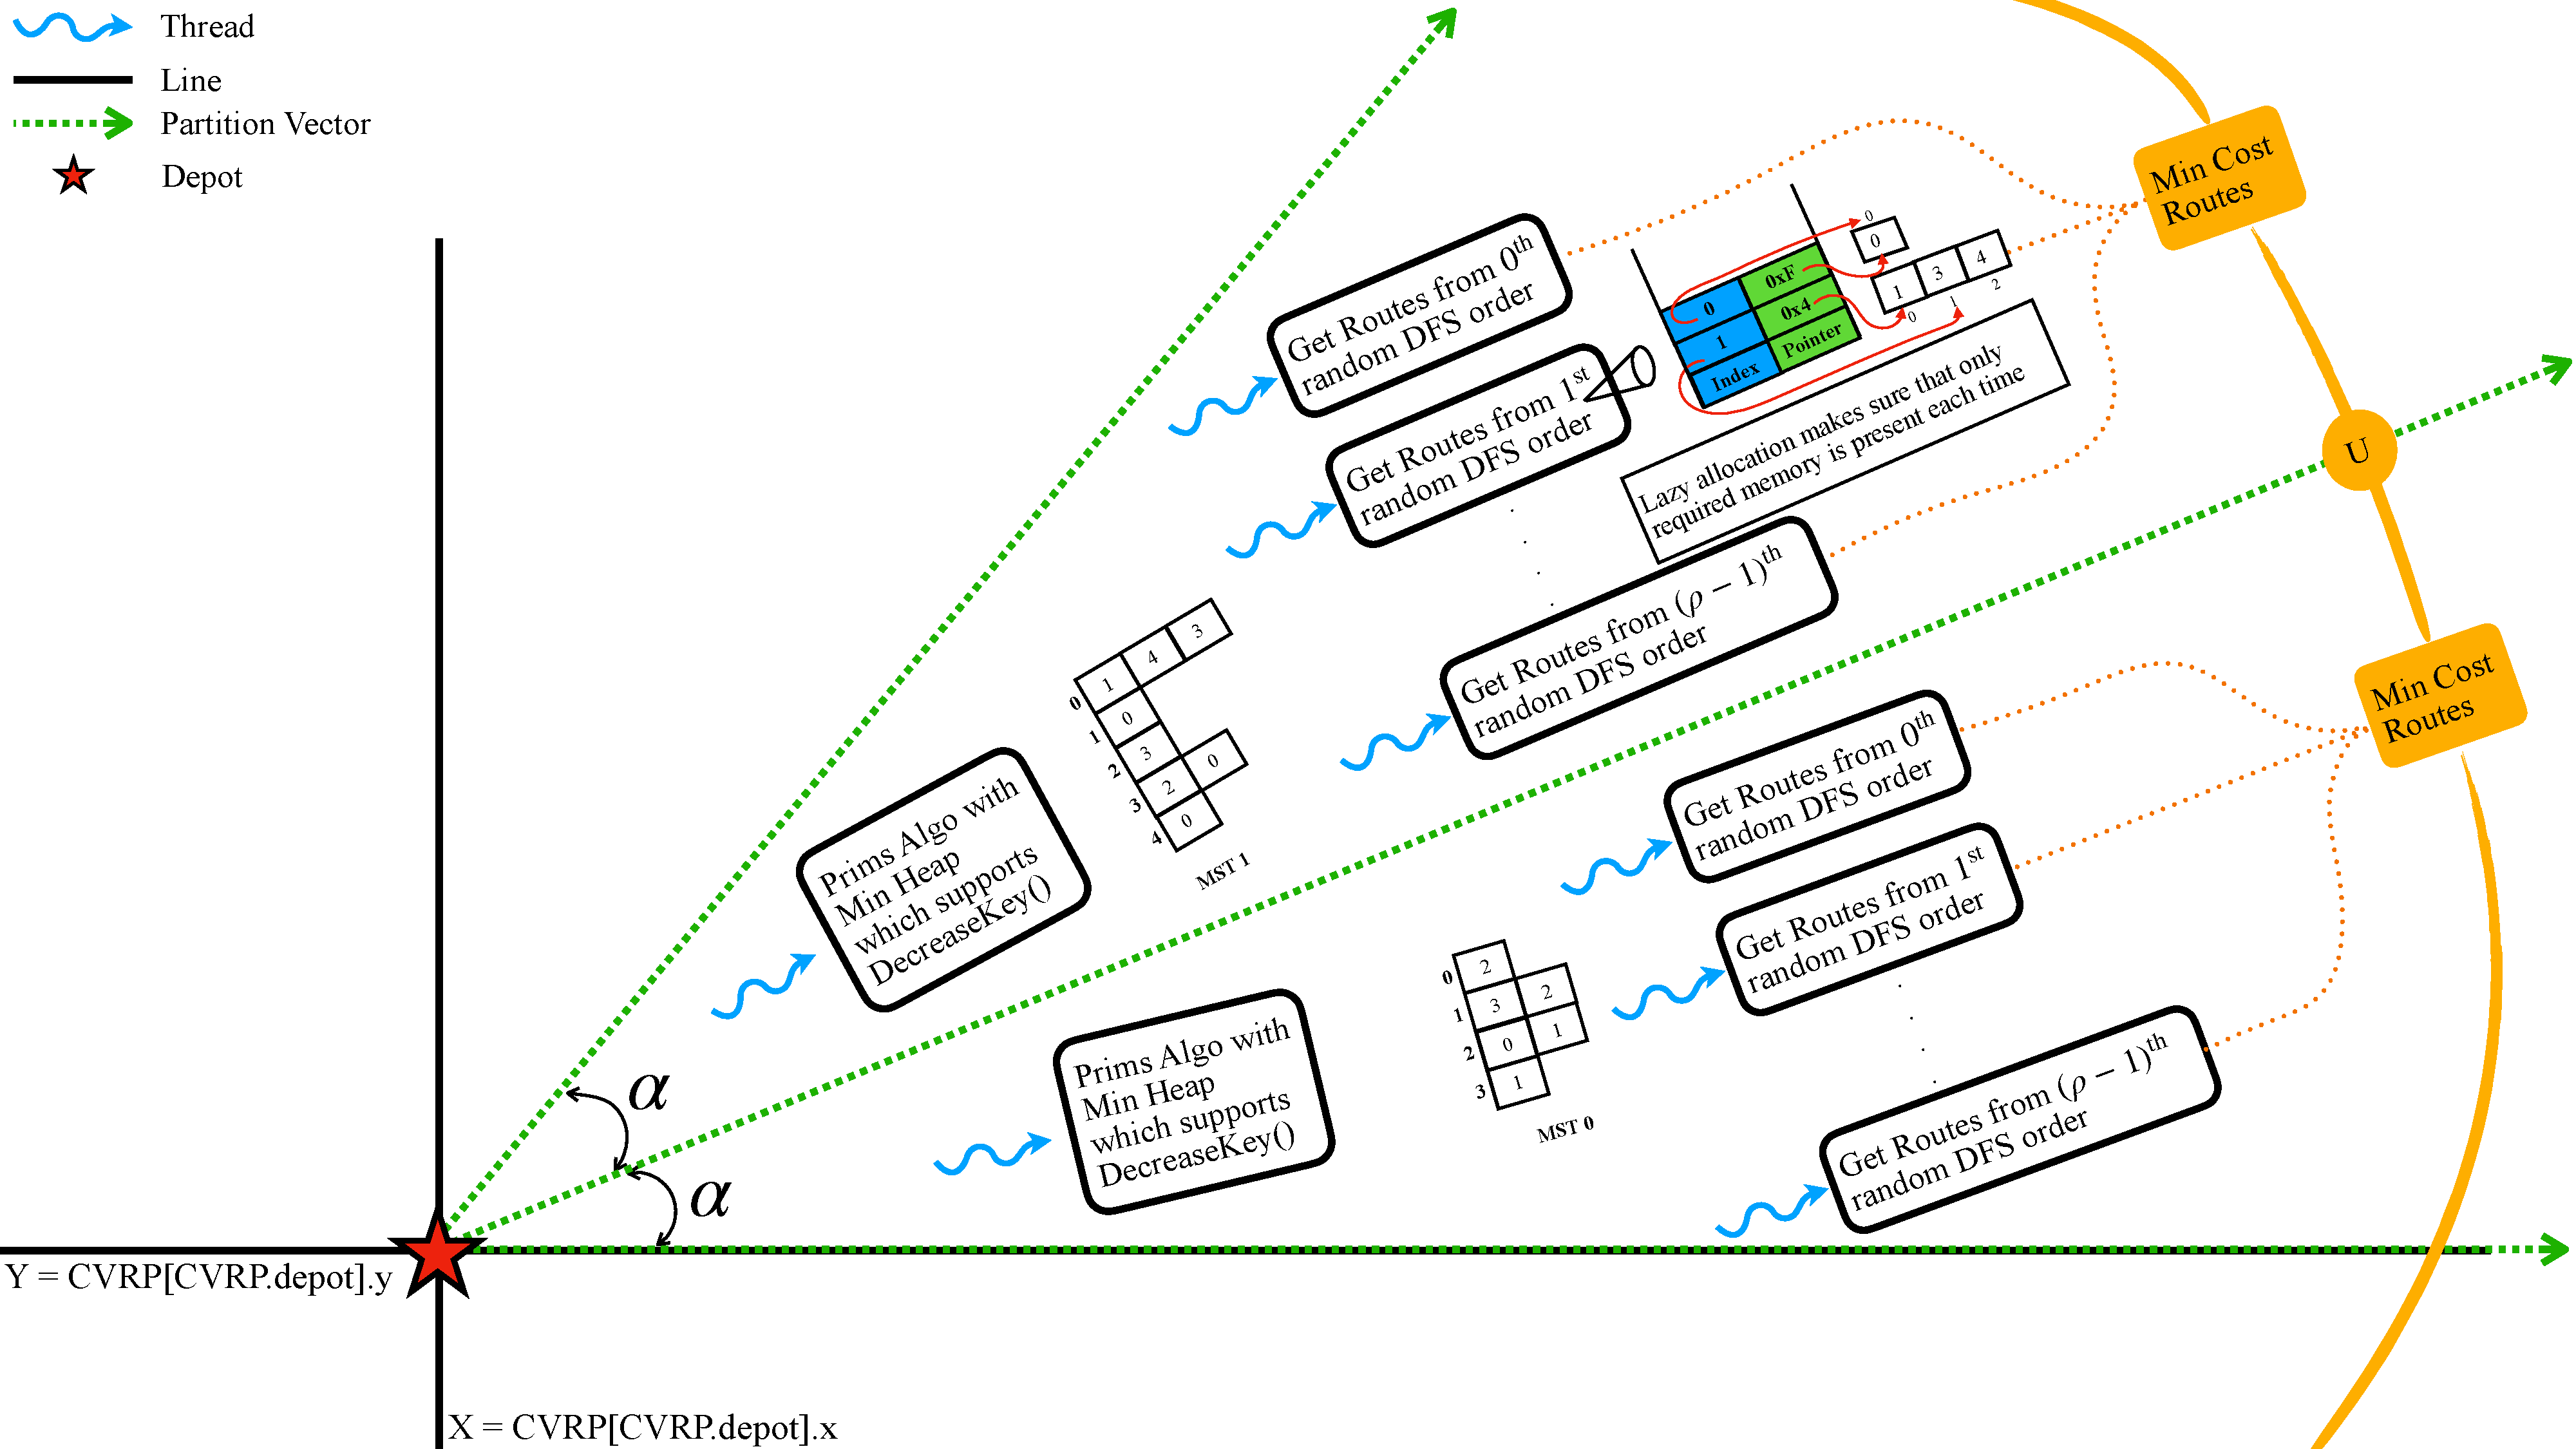
\includegraphics[width=\textwidth, height=0.4\textheight, keepaspectratio]{assets/multi-level-threading.pdf}
% \end{figure*}






